\documentclass[a4paper,10pt]{article}
\usepackage{graphicx}
\usepackage{sidecap}
\usepackage{subfig}

%opening
\title{A 3D viewer for ImageJ}
\author{B. Schmid, J. Schindelin, A. Cardona and M. Heisenberg}

\begin{document}

\maketitle
\setlength{\parskip}{0.3cm}


\begin{abstract}
In this paper, we introduce a tool for visualizing 3D datasets. Microscopy techniques in biology and medicine, like confocal microscopy, EM, MRI etc, often provide a stack of 2D images. For the investigation of these images, however, the two-dimensional view of the single slices is often not sufficient. We therefore developped a software for 3D visualisation, which allows to display the stacks optionally as surfaces, volume renderings or orthoslices. The software focusses on interactive, hardware-accelerated display of the stacks. Additionally, it offers possibilities for animation and movie recording, as well as an elaborate way to handle transformations of displayed bodies.
Three major aspects make this tool outstanding against existing software in the targeted field of usage:
\begin{itemize}
\item It is freely available and extensible.
\item It was developped for simplicity of usage.
\item It is incorporated into ImageJ \cite{imagej}, a prominent image processing software for microscopy data.
\end{itemize}
\end{abstract}




\section{Introduction}
Medical and biological imaging techniques often acquire 3D datasets in the form of stacks of 2D images. Confocal microscopy for example can be used to cut a \textit{Drosophila} brain virtually into slices of a few $\mu$m thickness and scans it. For many areas of research and application, the 2D view is not sufficient, however. For anatomists, e.g., it is vital to get an exact representation of the form and spatial relations of the tissue under study.

While there exists software for 3D visualisation, it suffers from several drawbacks: 3D software providing a comprehensive set of features is often proprietary and expensive, complicated in its usage or not suited for biological data. The tool we present does not share these shortcomings. While not restricted to this field of application, it was primarily designed for microscopic data. Its most relevant advantage however is its incorporation into ImageJ, which is one of the most wide-spread image processing packages in the field of microscopy. Users of ImageJ who already benefit from its numerous possibilities and plugins to process microscopic images, like filtering and deconvolution \cite{mbf}, can now visualize their data in 3D seemlessly, without the need of another software.

This paper is organized as follows: We first introduce briefly the technologies used for the implementation of the software. Subsequently, we show how the surface, volume and orthoslice views are created, as well as more information about the features of this software. Finally, more details about the implementation is provided.


\section{Technologies}
The technologies which were used in this work are ImageJ, Java and Java 3D.

\textbf{ImageJ} \cite{imagej} is used as underlying platform. There are several reasons for choosing ImageJ for this task: Using an image processing platform in general has the advantage that the developper does not need to take care about low-level actions like opening/saving images etc, since functionality like that is given by the chosen platform. The choice fell on ImageJ since it is by far the most widely used image processing software in the biological and medical field \cite{mbf}. Several reasons account for this:
\begin{itemize}
\item It is freely available and open source.
\item It consists of a compact core covering basic functionality, and is easily extendible to the user's needs by plugins.
\item There exists a active and competent community, which both serves as support via online forums and as developers for plugins of which hundreds can be found on the internet.
\end{itemize}
Using ImageJ facilitated our development as well as it facilitates the usage of the 3D viewer by scientists who are already familiar with ImageJ.

\textbf{Java} \cite{java} is a programming language which is platform independent. This means that our software runs on windows, unix and mac machines. ImageJ is written in Java.

\textbf{Java 3D.} To guarantee interactive 3D visualisation, hardware capabilities must be used optimally. Many 3D rendering tasks can nowadays be fullfilled by graphics cards, which frees the CPU and accelerates operations drastically. Java 3D \cite{java3d} is a technology which allows to use these hardware capabilities from within Java. An alternative to Java 3D would have been JOGL, a Java binding for OpenGL. However, in our eyes Java 3D is the more promising technology.



\section{3D Visualisation}
3D datasets can be represented in different ways. The options we implemented in this work are surfaces, volume renderings and orthoslices.
Starting point is a set of 2D slices which contain volumetric data, e.g. acquired by confocal microscopy. A stack like this can optionally be displayed as a three dimensional surface, orthoslices or as a volume rendering. These possibilities are described in more detail in the following paragraphs.
\subsection{Surfaces}
A surface is generally understood as the border between a volumetric body and its environment. Given a volumetric 3D dataset, constructing a corresponding surface is an ill-defined problem. In computer graphics, one often uses isosurfaces for this purpose. Isosurfaces assume that there is an intensity threshold which separates a body from its background. This border defines the isosurface, it therefore has the same intensity everywhere, which is also called its isovalue.

The most used representation of surfaces in computer graphics are polygon meshes, in particular triangular meshes. Java 3D provides methods to display triangle meshes and is capable of representing a surface internally as a triangle mesh.

To display volumetric data as a surface, the triangles defining the border between body and background have to be generated. One of the most commonly applied algorithms recruted for this purpose is the marching cubes algoithm \cite{lorensen87}, which we also utilized here.

A virtual cube "marches" through the volumetric stack and inserts triangles, according to the intensity values at the vertices of the cube (see figure \ref{fig:surface}a).

The resulting list of triangles are displayed, taking into account attributes like color and transparency. For a smooth, realistic representation, vertex normals are calculated and used for shading. An example of a 3D surface is shown in figure \ref{fig:surface}c, figure \ref{fig:surface}b shows how the surface is composed of triangles.

\subsection{Volume rendering}
Another method to visualize a set of 2D slices is volume rendering.
The general idea is to put the 2D slices one behind another. To avoid that the top slice obscure slices below, each voxel (volume element) is assigned a transparency value, which is dependent on its intensity value: Brighter voxels are more opaque, darker ones are more transparent.
In Java 3D, this technique can be implemented using textures: Each slice has a rectangular geometry, which defines the border of its texture. The texture itself is given by the set of 2D slices. (A tutorial about volume rendering in Java 3D can be found at \cite{volrend}.)
Figure \ref{fig:volume}c shows a volume rendering. To display coloured stacks, the transparency value of each voxel is calculated from the mean intensity of the red, green and blue color component.

To separate different channels in a double staining, our software allows to select the color channels to be displayed (figures \ref{fig:volume}a and \ref{fig:volume}b. Additionally, it provides the functionality to edit volumes via virtual scissors (figure \ref{fig:volume}d).

\subsection{Orthoslices}
The example of an orthoslice representation can be seen in figure \ref{fig:orthoslices}.
It consists of 3 orthogonal slices through the displayed volume. Together with the rotation capabilities, scrolling the slices through the volume offers a great way to follow neuritic fibres in brain tissue.


\subsection{Properties common to surfaces, volume renderings and orthoslices}
In the following, each item of the 3D universe, be it an orthoslice, a surface or a volume rendering, is called a body.
While all three kinds of bodies are different in general, they have several properties in common.
First, there is the behaviour they show on user interaction. Bodies can be rotated and shifted by the use of the mouse: The user can select a body through a click on it and then drag or shift+drag it to rotate and translate it respectively. (Without selecting a body, the same action causes the whole universe to be rotated/translated).
Several other properties are common to surfaces, volume renderings and orthoslices:
\begin{itemize}
\item color: It is possible to either show a body in its original color (as in the original set of the 2D slices) or to adjust its red, green and blue color component arbitrarily.
\item threshold: In case of a surface, this is the previously mentioned isovalue of the calculated isosurface. In case of volume renderings and orthoslices, it defines the lowest voxel value displayed. Darker voxels are omitted from the 3D rendering.
\item transparency value
\item channels: The color channels of the original 2D slices, which should be used for displaying the 3D body (see figure \ref{fig:volume}a and \ref{fig:volume}b).
\end{itemize}

The user can either set these properties when adding a body to the 3D universe, or she can change existing properties lateron.

\subsection{Several bodies in the 3D universe}
For several reasons, it is desirable to show more than one body in the 3D world.
Figure \ref{fig:multiple} shows as an example a 3D world with an isosurface of a fly brain wholemount, together with the volume rendering of some coloured neuropiles (lobula, mushroom bodies and antennal lobes).

Having more than one body in the 3D world comes along with some difficulties for the implementation. To be useful, it must be possible to interactively transform each body individually, as well as to transform the 3D universe as a whole. As stated previously, the mechanism is implemented in the following way: If the user selects an individual body by clicking on it (the selection shows up by a red bounding box), only the selected body is transformed, the others keep their position and orientation. If no body is selected, the whole universe is transformed.
More details about how this is implemented in the software can be found later in the implementation details.

\subsection{Handling transformations}
There exist two ways to transform a body in the 3D universe. The first one, which has already been mentioned, is by direct user interaction via the mouse. Transformations are restricted to translation and rotation. (Scaling, or zooming, is possible as well, but not on the level of individual bodies).

Next to direct interactions via the mouse, transformations can be specified explicitly for each body, in the form of a 4x4 matrix. The user can set a transformation, she can concatenate the current transformation with a newly specified one, she can store the current transformation of the body to an external file and reload it.

This possibility to specify defined transformations on the level of individual bodies can for example be used to investigate and visualize the results of 3D image registration. Image registration is the transformation of a model image in such a way that it matches a reference image \cite{jenett2006}. Its purpose is for example the creation of an average staining out of images obtained from equally stained tissue of different individuals within one species. One loads the template image into the 3D world, without specifying a transformation, and subsequently the model image, with the transformation calculated by a registration algorithm. This enables one to manually judge the quality of the registration.

\subsection{Animation and movie recording}
Our software allows to animate the 3D universe. It is possible to record a movie of such an animation. The result is a stack of 2D images, which show subsequent frames of the animation (figure \ref{fig:animation}. This stack can be saved in video format, e.g. by ImageJ's avi exporting function. Video files like this one can be easily incorporated in powerpoint presentations.

\subsection{Landmark sets and registration}
Each body in the 3D world may optionally own a landmark set, i.e. a set of named points. Creating landmark sets is very much facilitated in our viewer: Using ImageJ's point selection tool and clicking on a body initiates landmark creation. A list with all landmarks shows up, offering the possibility to rename or
remove different points, or to highlight them in the 3D view. Landmark sets can
be displayed or hidden, saved to disk and be reloaded again.

Landmark sets are very helpful if one simply wants to label special positions in a tissue. However, they are also of particular use for landmark based registration. As pointed out above, image registration or alignment is very important for biomedical image analysis, e.g. for comparison or collocalisation studies. 

Many papers which aim for fully automated image registration. Depending on the image quality, however, fully automated methods offen don't obtained the desired results. On the other hand side, landmark creation in a 3D view, particularly using orthoslices, is so straightforward, that we implemented a registration algorithm based on manual landmark selection. At the moment, this is a rigid registration method first introduced in // TODO, but we aim to add more sophisticated techniqes in the future.

After initiating registration via the menu, a dialog pops up, asking the user for a model image and a reference image (the one the model is aligned to). Subsequently it guides the user through the process of landmark creation of both reference and model image, and calculates a global rigid transformation which best transforms the landmark set of the model image on that of the reference image. The transformed model can optionally be exported into a stack of 2D slices and stored as an ordinary tiff image.



\section{Implementation aspects}
\subsection*{Integration into ImageJ}
As mentioned previously, ImageJ consists of a tight core covering basic image processing functionality. This core can be extended individually by installing additional plugins, either developped on one's own or obtained from third parties.
To meet ImageJ's structure, the 3D viewer was also implemented as a plugin. It can easily be installed by downloading it and placing it into ImageJ's plugins directory.

\subsection*{Java 3D scene graph}
The scene graph is an arrangement of 3D objects in a tree structure that completely specifies the content of a virtual universe, and how it is to be rendered. It consists of nodes which specify the 3D objects by defining their geometry, appearance, location and transformation. There exist also nodes which define the properties of the universe like sight sources and sound. \cite{java3dtut}

Different types of nodes exist which have different function: The most prominent ones are:
\begin{itemize}
\item BranchGroup: A node that is capable of being the root of several subtrees.
\item TransformGroup: A Node that transforms the subtree below by a specified transformation.
\item Switch: A node having several child nodes, whose display can be toggled (i.e. which can be switched on and off).
\item Shape3D: A node representing a body in the 3D world. A Shape3D is specified by its Appearance and Geometry objects.
\item Geometry: Defines the geometry of the corresponding Shape3D, e.g. its vertex coordinates. In case of an isosurface, the geometry holds the triangle mesh, in the case of a volume rendering or orthoslices, it holds a set of rectangles.
\item Appearance: Defines several attributes of a Shape3D which influence its display, like color, transparency, textures etc.
\end{itemize}

Parts of the scene graph of the 3D viewer are shown in figure \ref{fig:scenegraph}. It particularly shows the path from the topmost root node to an attached Shape3D representing a surface. The structure is intended to elucidate the interplay of the different TransformGroups, which allows the rather complex transformation handling in the viewer. The nodes have the following meaning:

\begin{description}
\item[TG scale:] TransformGroup for global scaling. Acts either on user interaction (zooming) or automatically to fit a body into the 3D universe.
\item[TG rotate:] TransformGroup for global rotation. Acts on user interaction when no body is selected.
\item[TG translate:] TransformGroup for global translation. Acts on user interaction when no body is selected.
\item[TG center:] TransformGroup for centering displayed bodies in the universe. Each time updated when a new body is added to the universe.
\item[BG scene:] BranchGroup which holds a subtree for each displayed body.
\item[BG content:] Root BranchGroup of a body's subtree.
\item[TG l\_translate:]  TransformGroup for local translations. Acts on user interaction when a body is selected.
\item[TG l\_rotate:] TransformGroup for local rotation. Acts on user interaction when a body is selected.
\item[Switch bcSwitch:] Switch which holds next to the body's Shape3D a optionally displayable coordinate system and the bounding box which shows up on selection.
\item[Shape3D surface:] Shape3D which represents the surface.
\end{description}



\section{Availability}
The 3D viewer can be downloaded on our homepage at http://www.neurofly.de under Downloads $>$ ImageJ $>$ ImageJ 3D Viewer. On the same site, comprehensive documentation can be found, together with a screen movie demonstrating all the features of the viewer.




\bibliographystyle{plain}
\bibliography{../bibliography}



\begin{figure}[m]
  \centering
  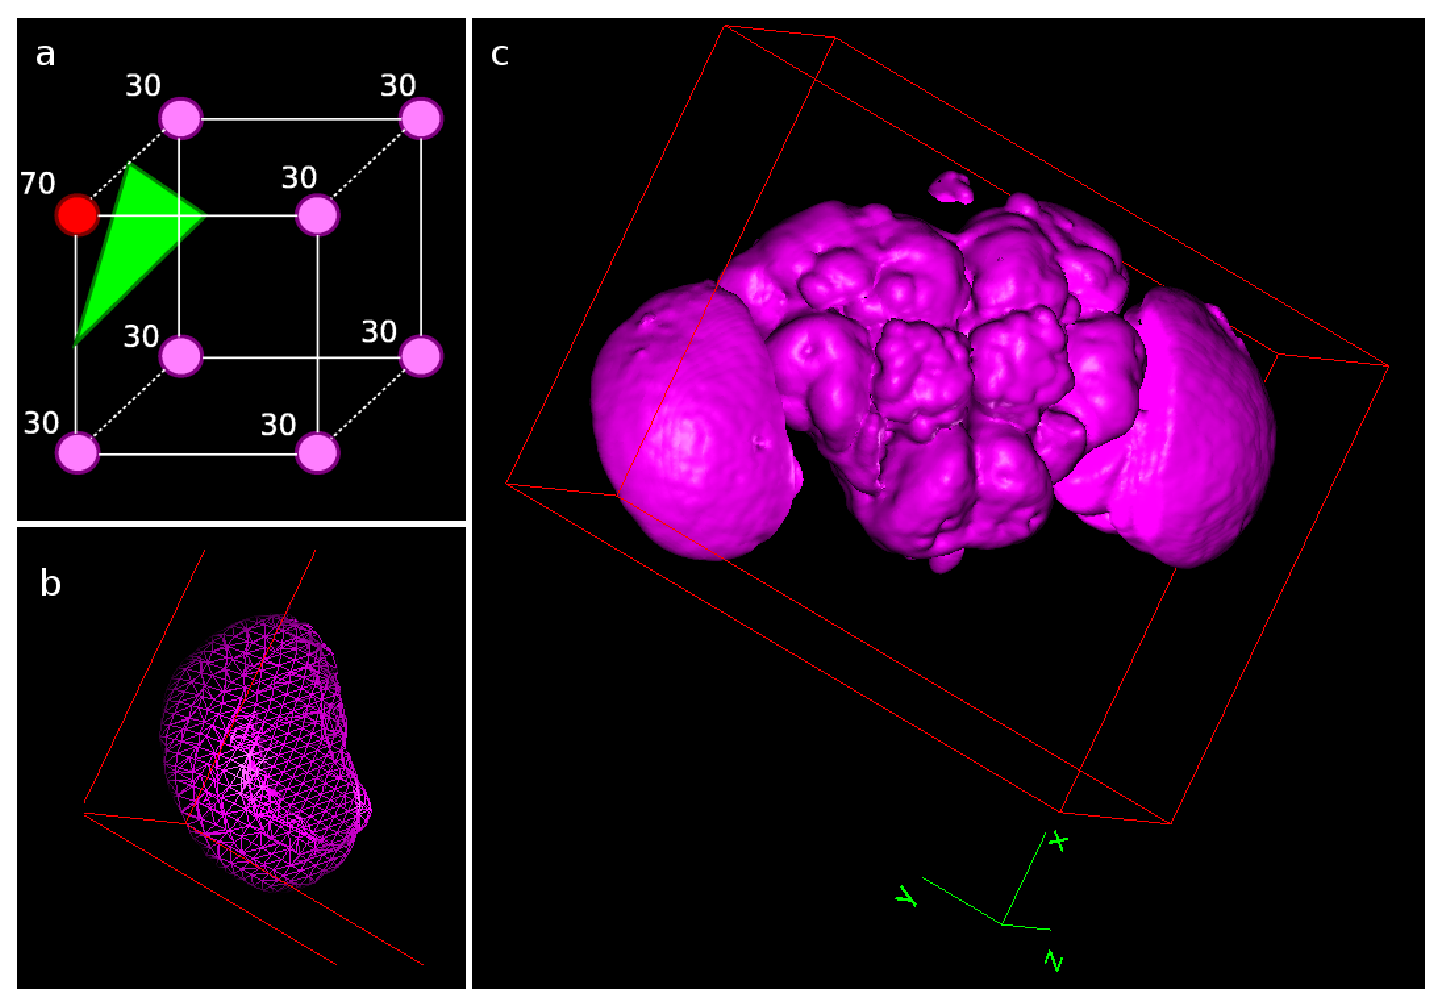
\includegraphics[width=\textwidth]{images/surface_montage.eps}
  \caption{Isosurface. Isosurfaces can be generated by the marching cubes algorithm. A cube is moved to the through the volume. The vertices of the cube are given by 8 neighbouring voxel values. Dependent on these 8 values, triangles are inserted at each position (a). The isosurface shown in magenta (c) was generated from a stack of 2D slices showing a fly brain. The images were obtained by confocal microscopy. In green one can see an optionally displayable coordinate system which indicates the origin of the original stack. In red one can see a bounding box which indicates that the brain is selected. In (c), the triangle mesh of the one of the optic lobes is shown.}
  \label{fig:surface}
\end{figure}



\begin{figure}[m]
\centering
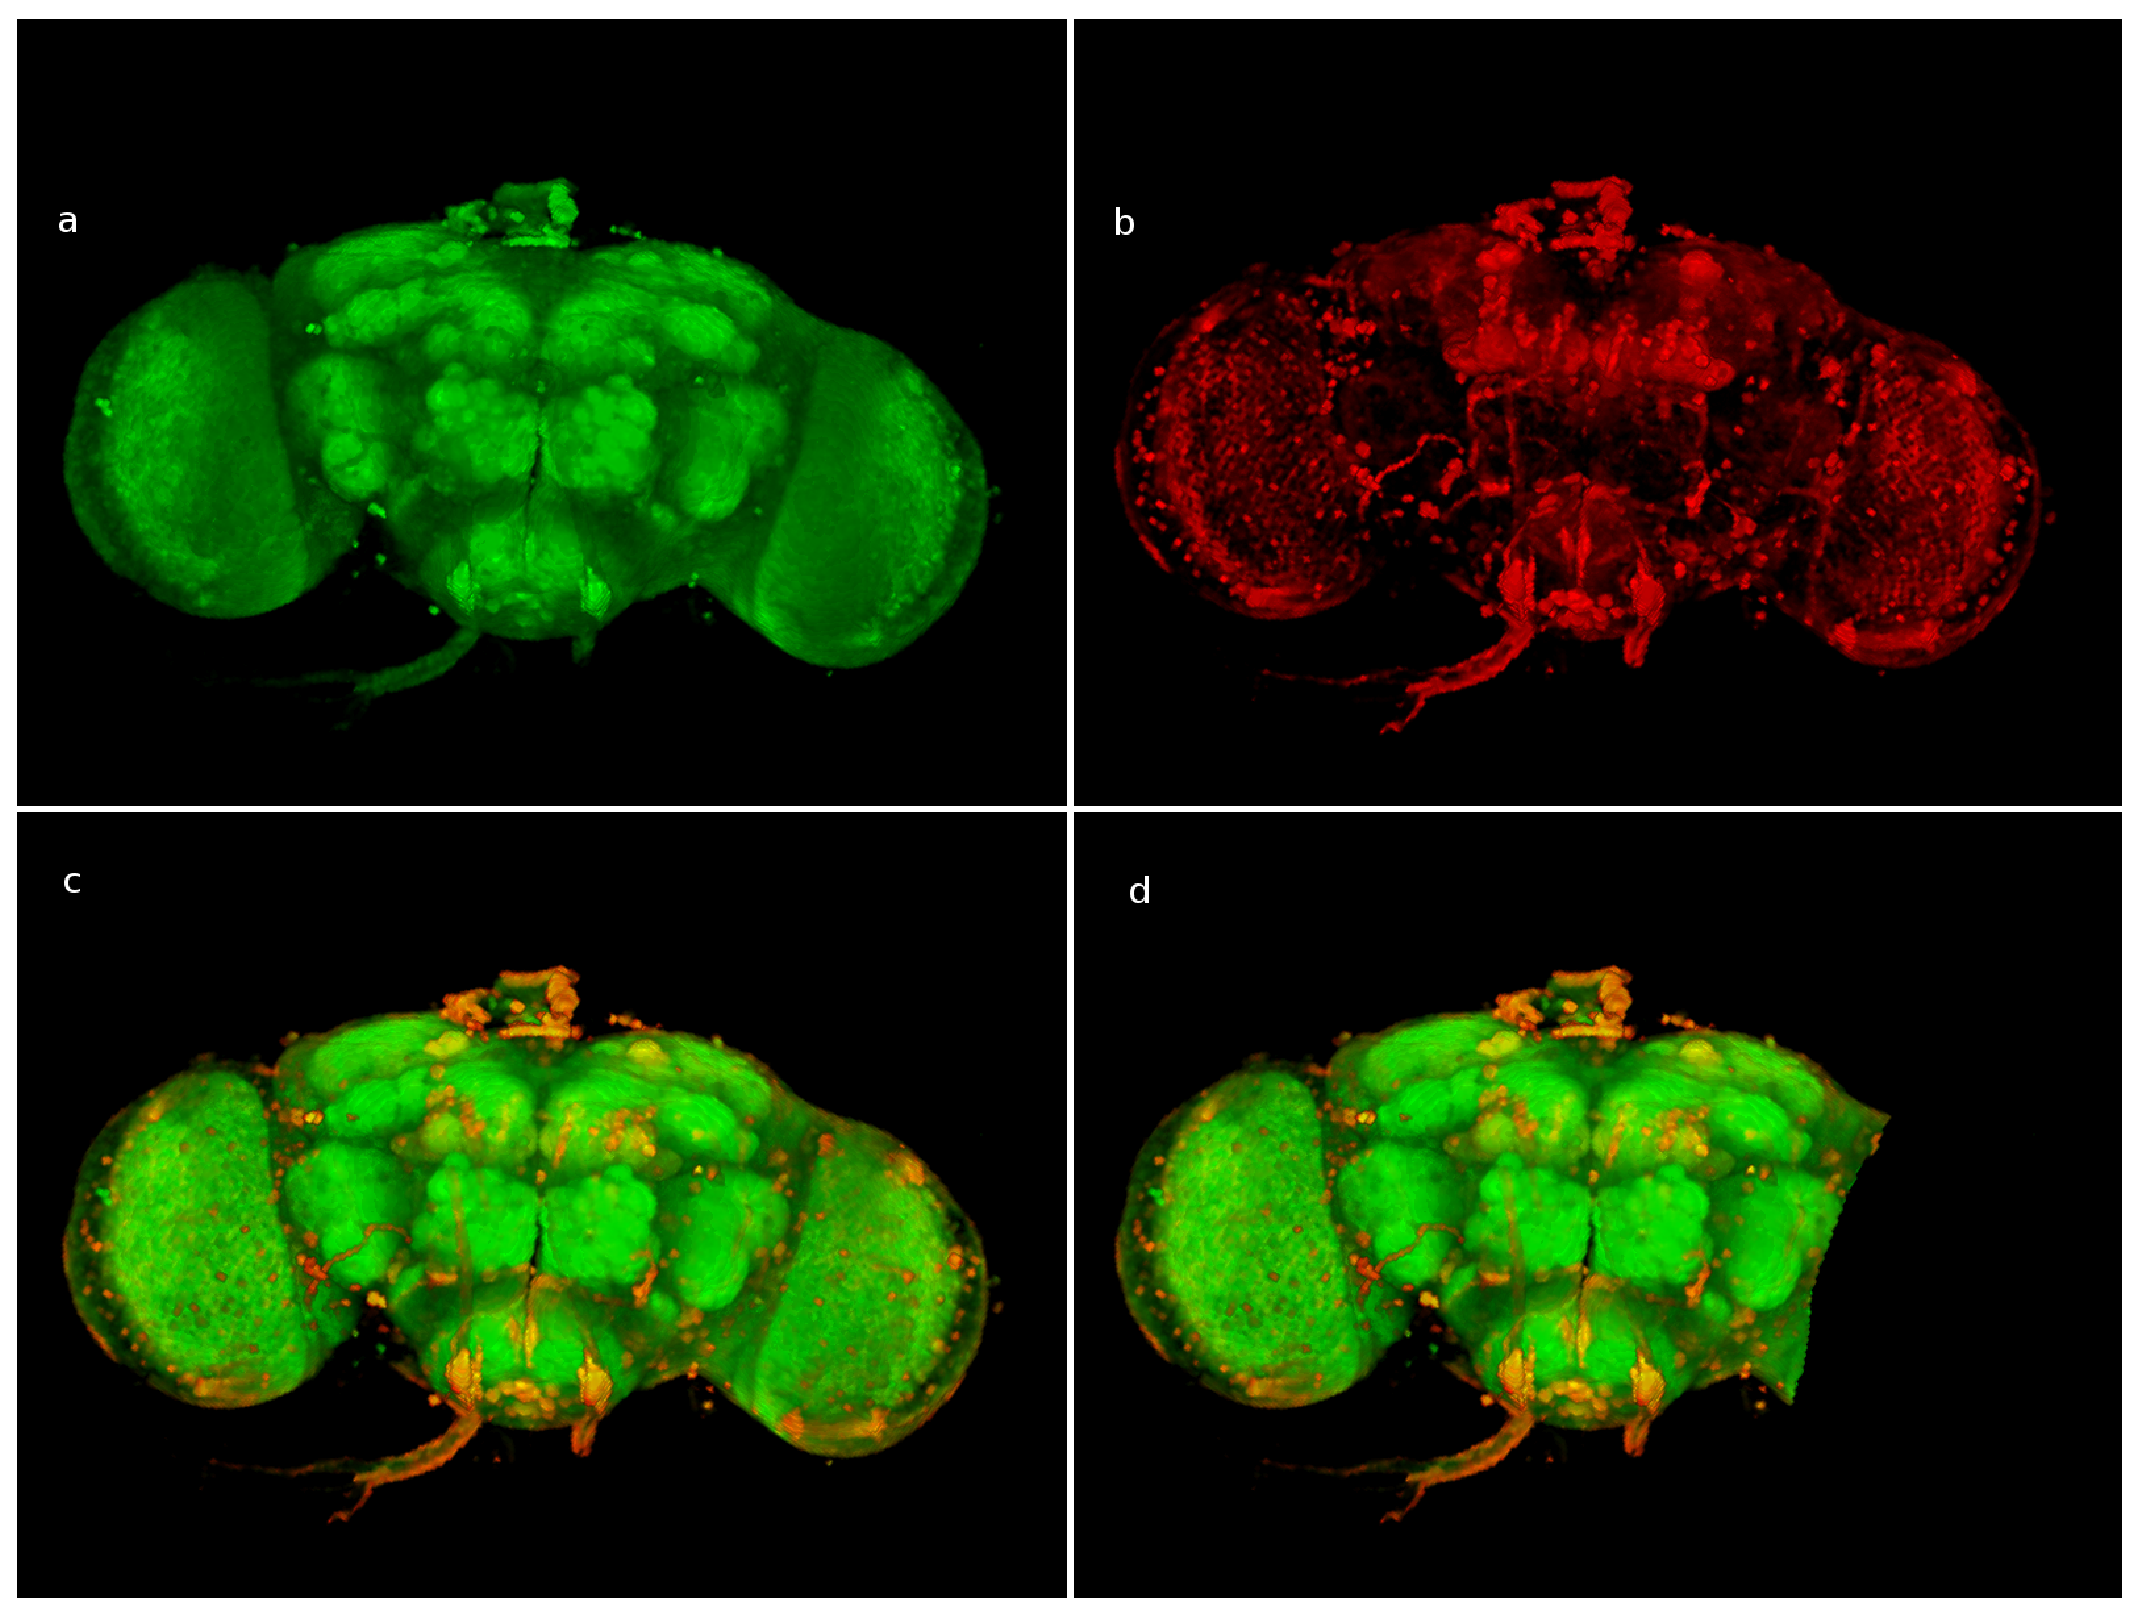
\includegraphics[width=\textwidth]{images/volume_montage}
% \centering
% \subfloat[]{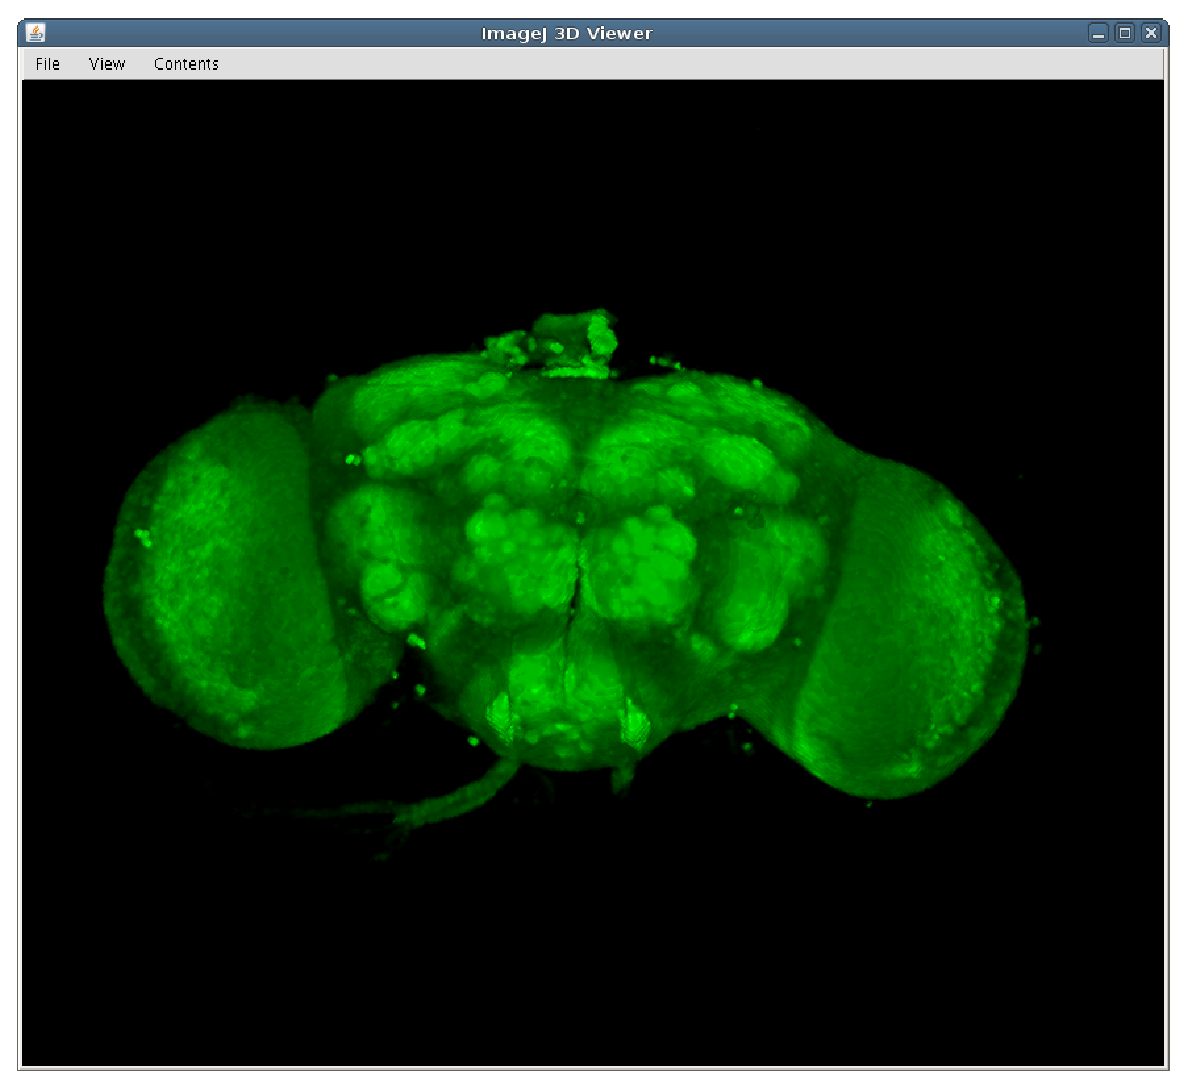
\includegraphics[width=0.45\textwidth]{images/volume_green}}
% \hspace{3mm}
% \subfloat[]{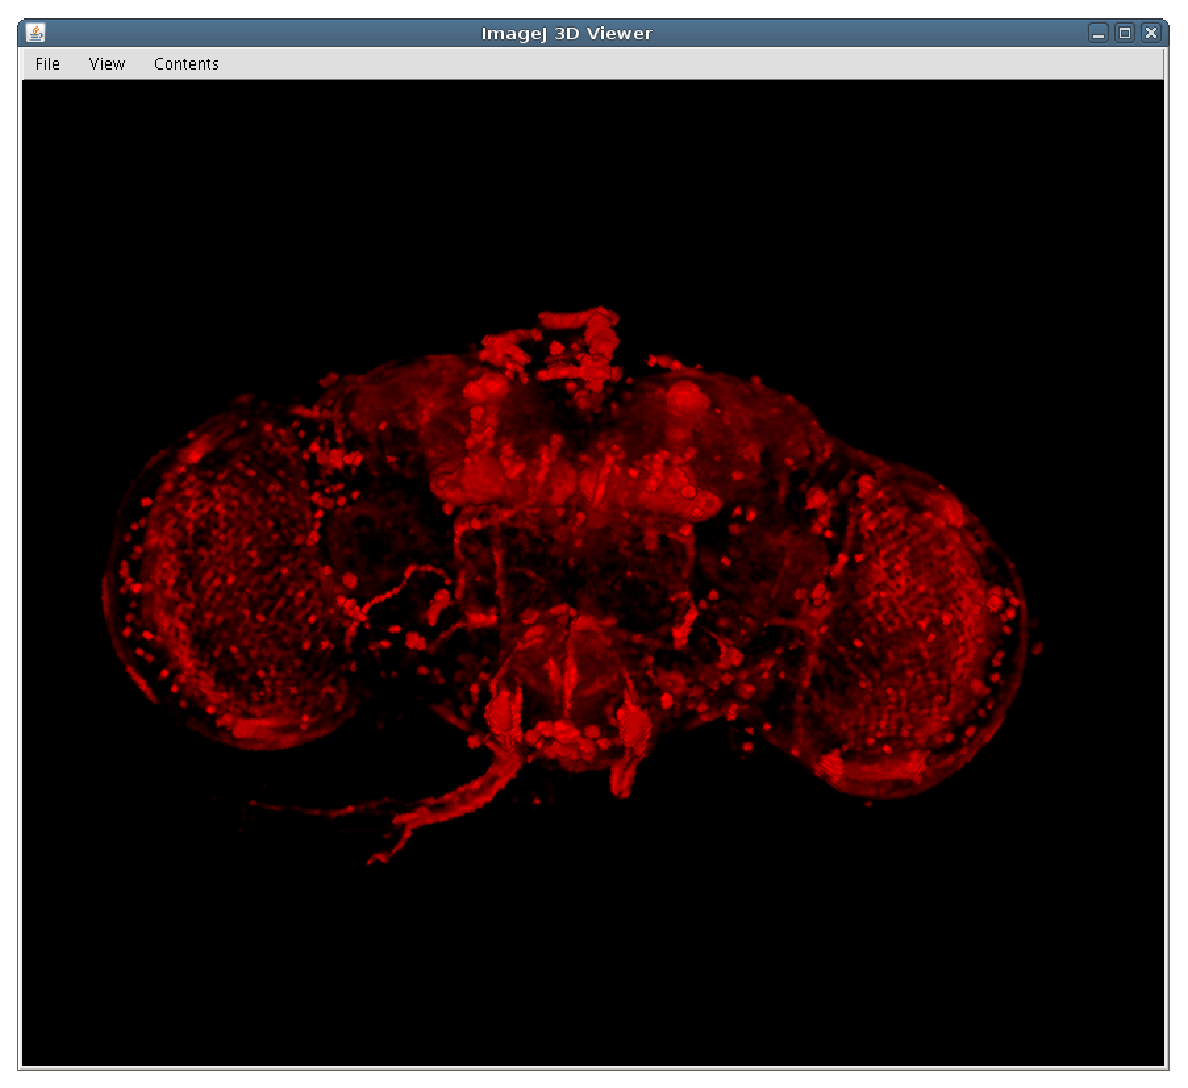
\includegraphics[width=0.45\textwidth]{images/volume_red}} \\
% \subfloat[]{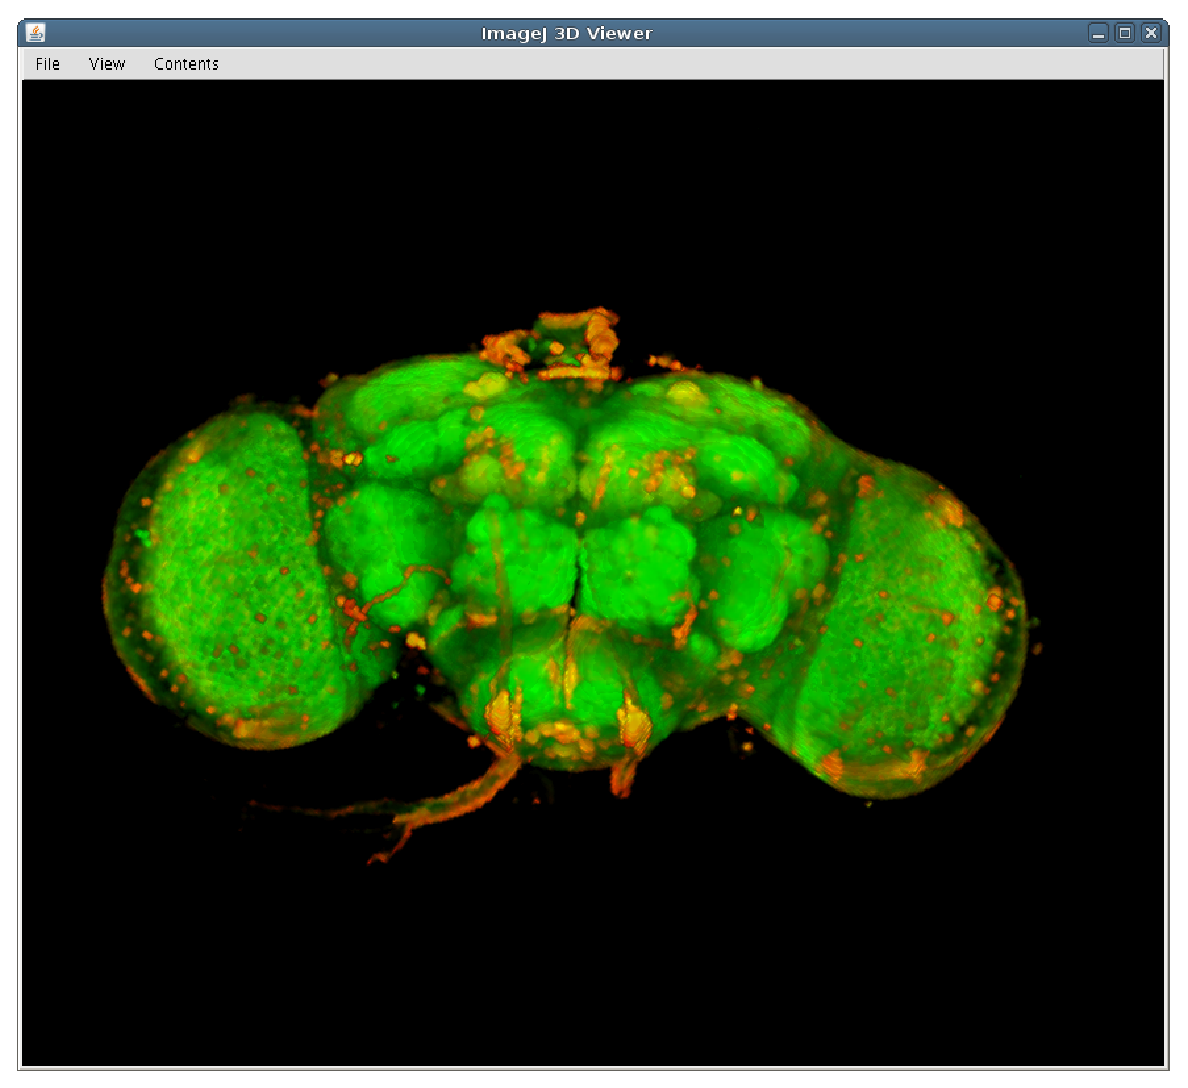
\includegraphics[width=0.45\textwidth]{images/volume}}
% \hspace{3mm}
% \subfloat[]{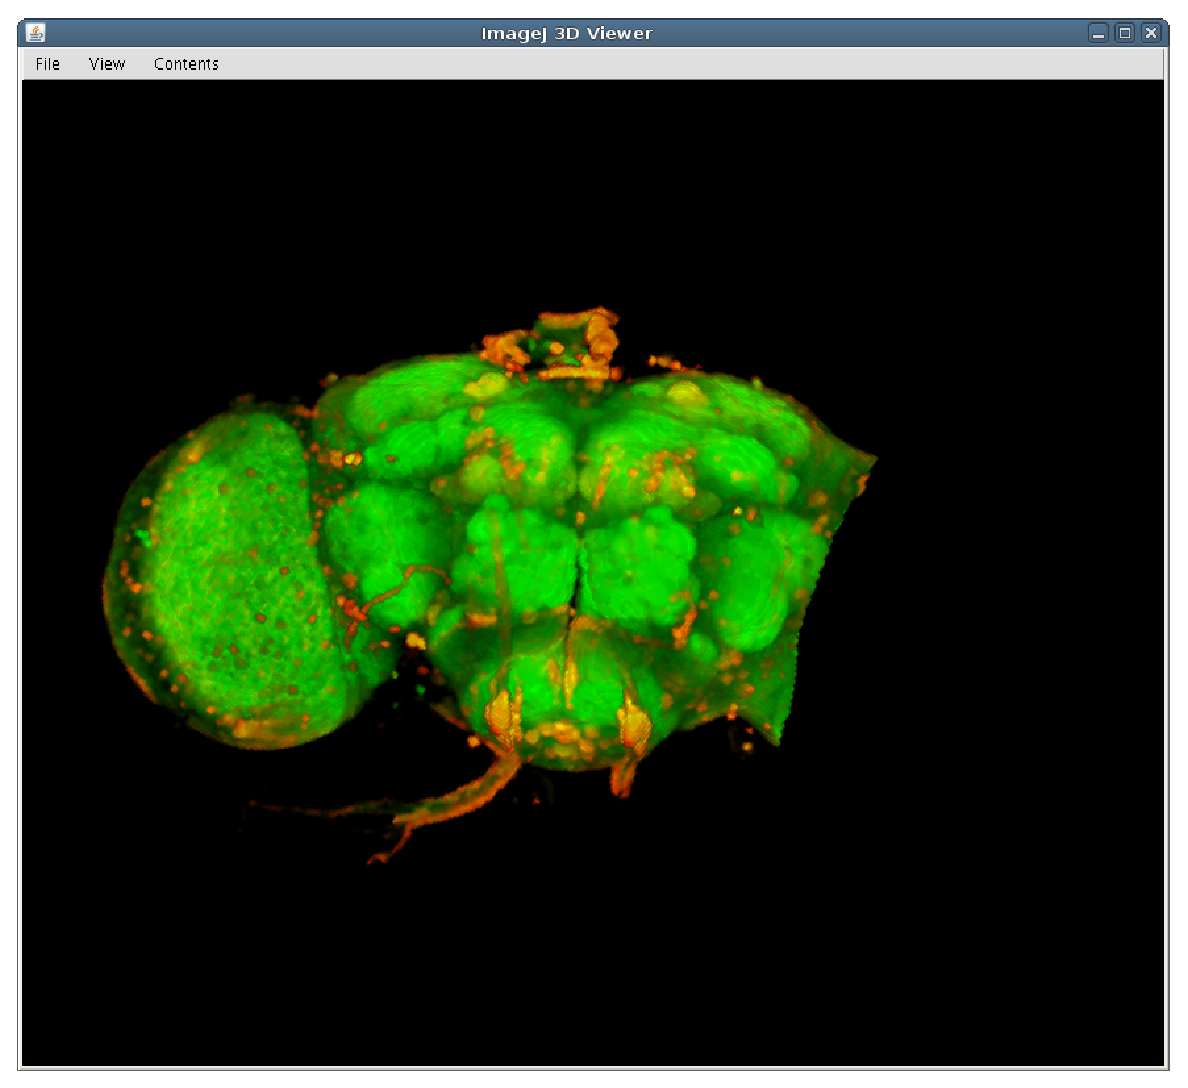
\includegraphics[width=0.45\textwidth]{images/volume_edited}}
\caption {Volume rendering. This volume rendering shows also a fly brain. Alexa 488, a green dye, was used as a reference staining to colour the whole brain. Cy3, a red dye, was used to stain some specific brain regions. Where boths dyes coincide, the tissue shows up yellow. The viewer allows to specify the channels which should be displayed. (a) shows the green channel, (b) shows the red channel, (c) shows the red and green channel combined. The viewer allows additionally to edit volumes. (d) shows the same brain, with the right optic lobe cut off via the viewer's volume editing tool.}
\label{fig:volume}
\end{figure}

\begin{figure}[m]
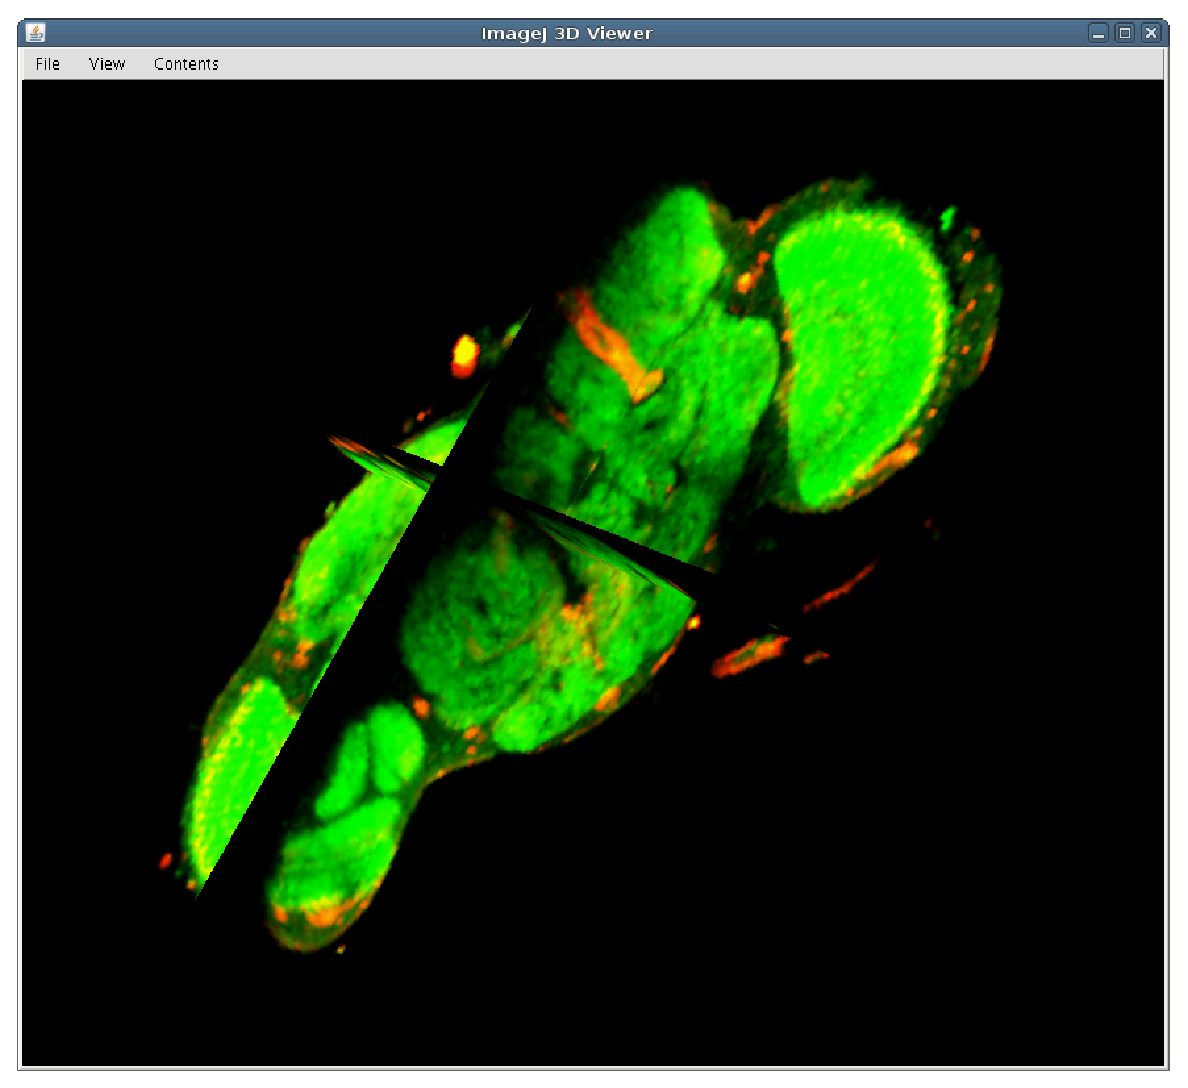
\includegraphics[width=\textwidth]{images/orthoslices.eps}
\caption{Orthoslices. Orthoslices are 3 orthogonal slices through the volume. Shown here is the same fly brain as in figure \ref{fig:volume}. The slices are chosen in such a way that a section through the right peduncle, which was stained by the red and green dye, is visible.}
\label{fig:orthoslices}
\end{figure}

\begin{figure}[m]
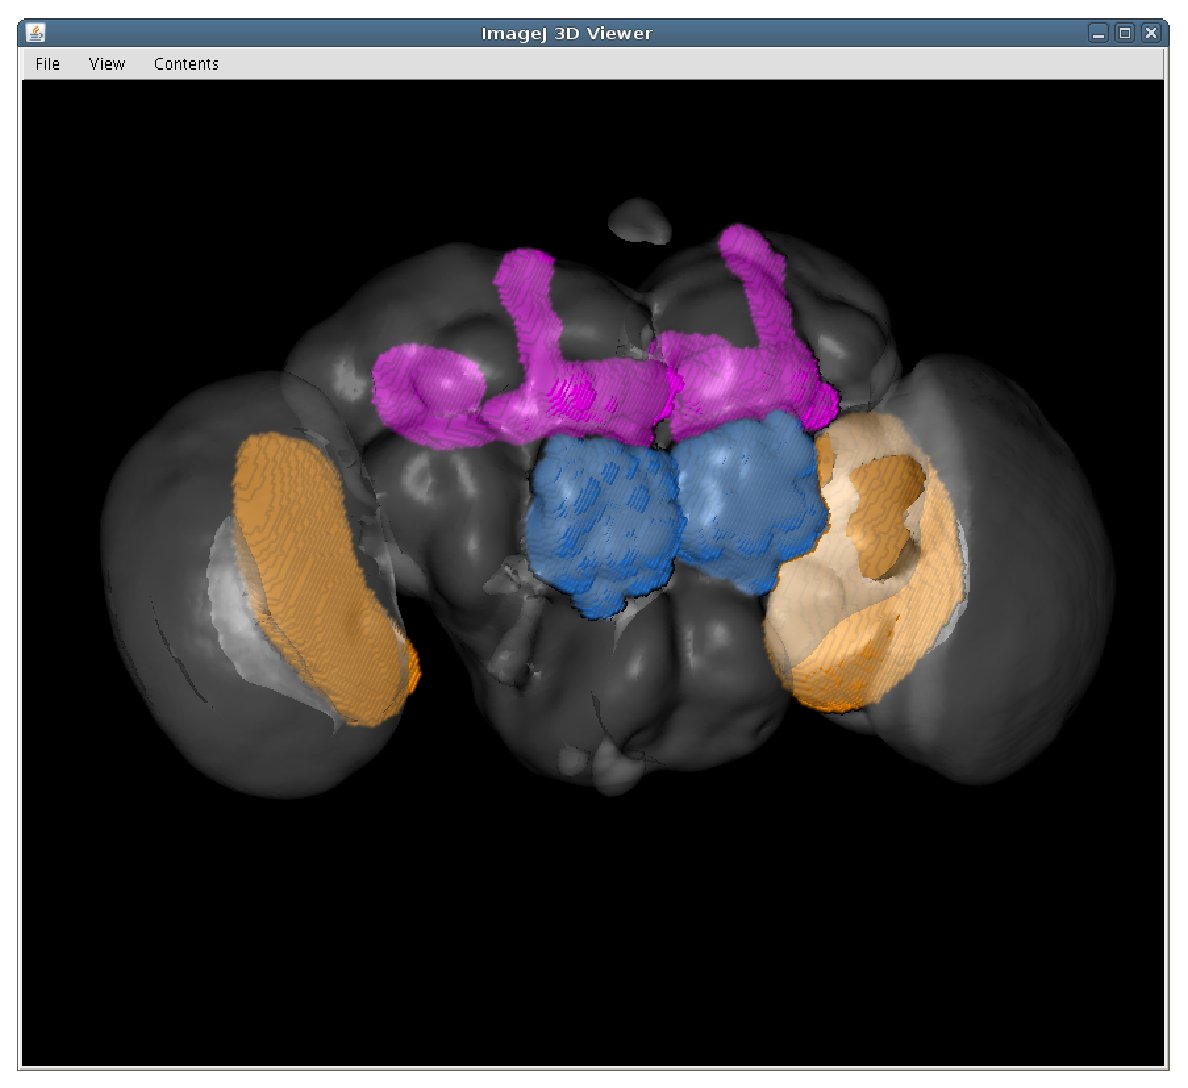
\includegraphics[width=\textwidth]{images/multiple.eps}
\caption{Multiple bodies. The isosurface shown in figure \ref{fig:surface} is shown here in lightgray and a transparency value of 0.5. Additionally, the volume rendering of another stack is displayed, which shows lobula (orange), mushroom bodies (magenta) and antennal lobes (blue) of the same brain.}
\label{fig:multiple}
\end{figure}

\begin{figure}[m]
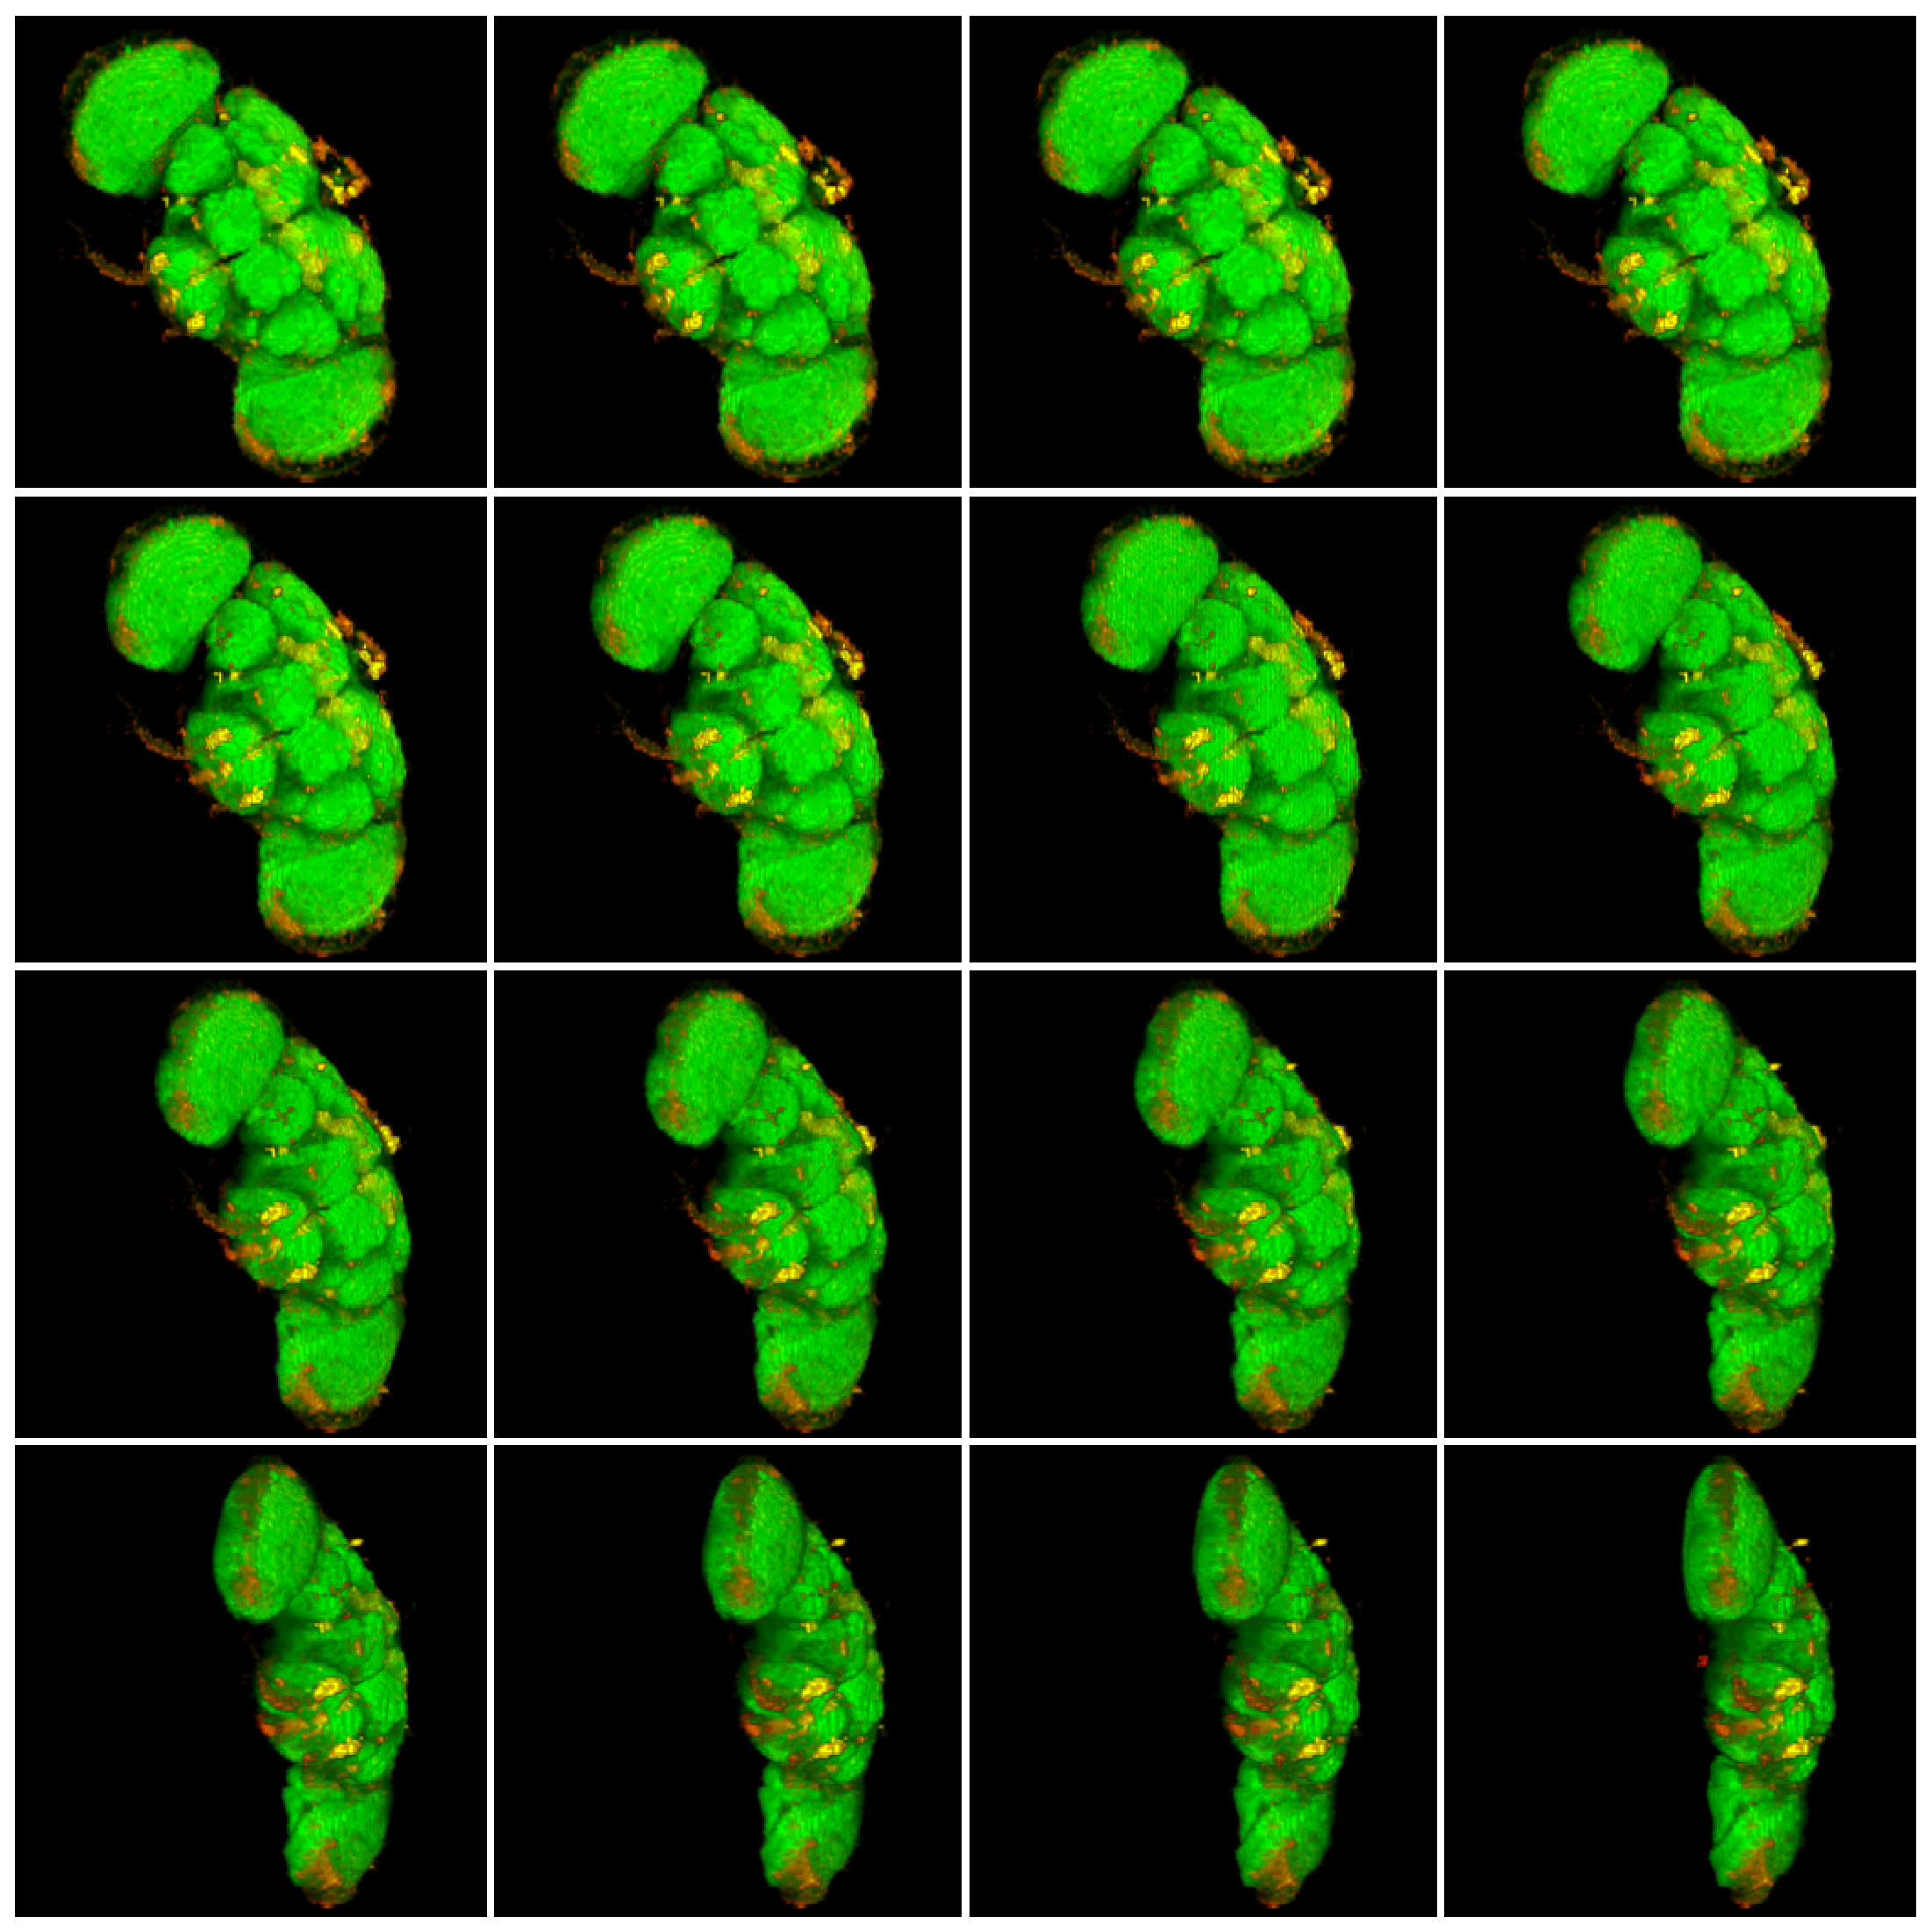
\includegraphics[width=\textwidth]{images/animation.eps}
\caption{Animation. The image sequence here shows a rotation of about 90 degree. An animation like this can be recorded and results in an image stack, which can be saved in a video format like AVI.}
\label{fig:animation}
\end{figure}

\begin{figure}[m]
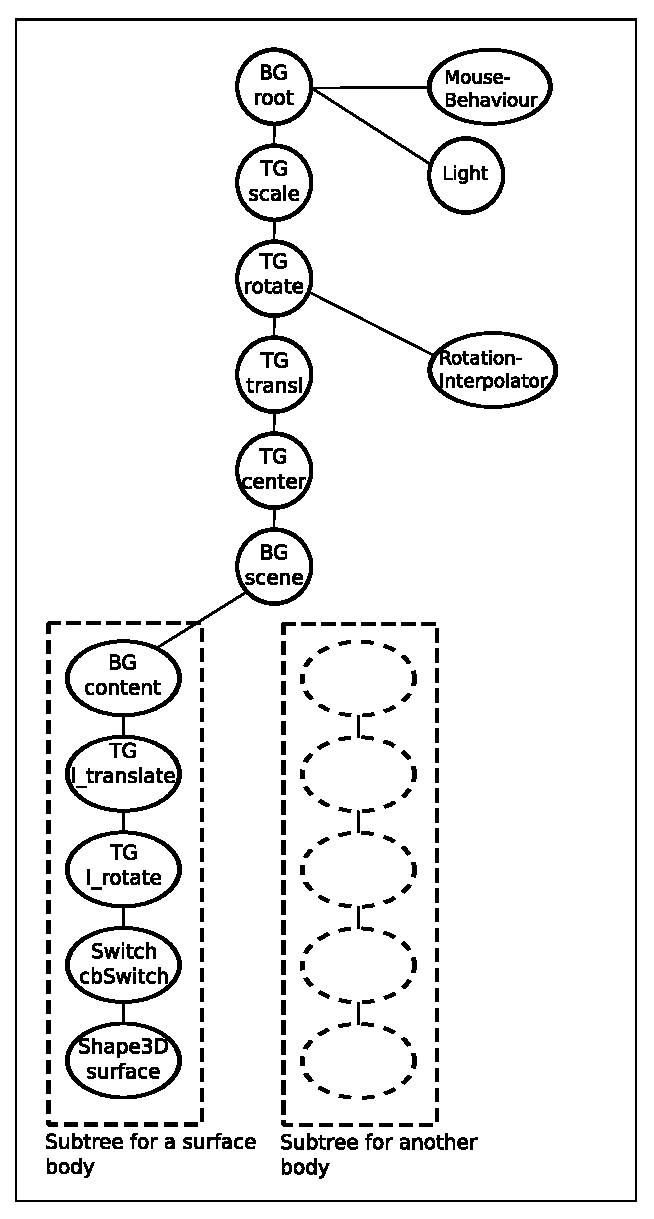
\includegraphics[width=0.7\textwidth]{images/scenegraph.eps}
\caption{Part of the scenegraph of the 3D viewer. Shown here is an example path from the root node to a surface node. For more information about the meaning of the nodes see the text.}
\label{fig:scenegraph}
\end{figure}

\end{document}

